
\section {Evaluation}

In this section we  show that  the  separation of the data  plane from
control and management operations in  the \system architecture results
in a  system where network functions  can be deployed with  very small
overhead.   Compared with a    conventional deployment that  relies on
routing for  service chaining, \system adds a  network round trip time
for session setup, which  can be  easily  and safely eliminated  in an
enterprise network if the  session setup information is piggybacked in
TCP  syn    packets,      we  describe      this optimization       in
\S\ref{sec:3way-handshake}. Moreover, we show that \system can sustain
throughput  at line  speed    in a   40   Gbps testbed  and    present
microbenchmark results for  the overheads introduced for table lookup,
rule insertion, and header rewrite.   We also show measurement results
for latencies introduced during  session  setup when multiple  network
functions are on the  session path and  latencies for flow  migrations
under different order preserving semantics.


%In our evaluation, we demonstrate that:
%\kelvin{Need to add more eval!}
%\begin{itemize}
%\item The system can sustain very high throughput
%\item The system has extremely low latency for flow migrations
%\end{itemize}

We used two  dedicated testbeds for  the performance  evaluation, with
the following configuration:  (i) one L2 switch  with 16  1Gbps ports,
and five  {\em mid-range} workstations,  each with one Intel Quad-Core
Xeon 3.7GHz processor,  32GB of memory, and two  1Gbps NICs; and  (ii)
one L2 switch with four 40Gbps ports, and four {\em high-end} servers,
each with two Intel 8-Core Xeon 2.2GHz processors, 64GB of memory, and
one  40Gbps NIC.   We  conducted throughput  stress tests in  the four
high-end servers, and unless specified, all the other experiments were
performed in setting (i).

\subsection{Throughput }

We first show that  \system can  sustain throughput  at line speed  in
40Gbps links using a vanilla Linux kernel and  1500-byte packets.  The
throughput  numbers  were  obtained  from   {\tt   iperf}~\cite{iperf}
executions  on  three  {\em high-end}  machines   connected  on a line
topology client--middlebox--server.  Since  the high-end machines have
only one NIC  each, we configured virtual interfaces  on  the NICs and
connected them to different IP subnets.  As a baseline for comparison,
we  enabled  IP routing  on the  middlebox  on  the  same topology and
removed the \system kernel modules on the three machines. We also show
the throughput results for  three other  configurations: first, a  VPN
tunnel  between  the middlebox  and the  server; second,  the same VPN
tunnel with compression enabled (VPN+OP); and third, a software switch
(OVS) performing network address  and port translations.   VPN tunnels
have been proposed  as a solution  for outsourcing virtualized network
functions to the cloud~\cite{Aplomb}.  The OVS results are included to
show the throughput gains of  having a dedicated kernel implementation
for \system.


\begin{figure*}[ht]

\centering
% 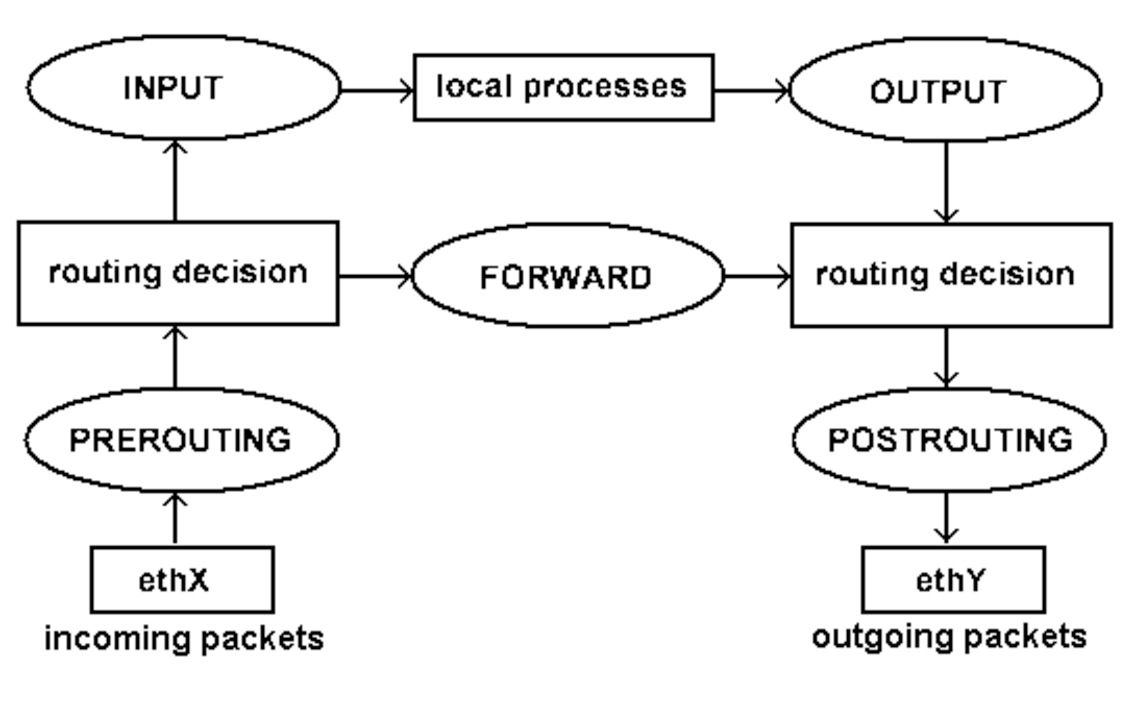
\includegraphics[scale=0.25]{figures/netfilter.pdf} 
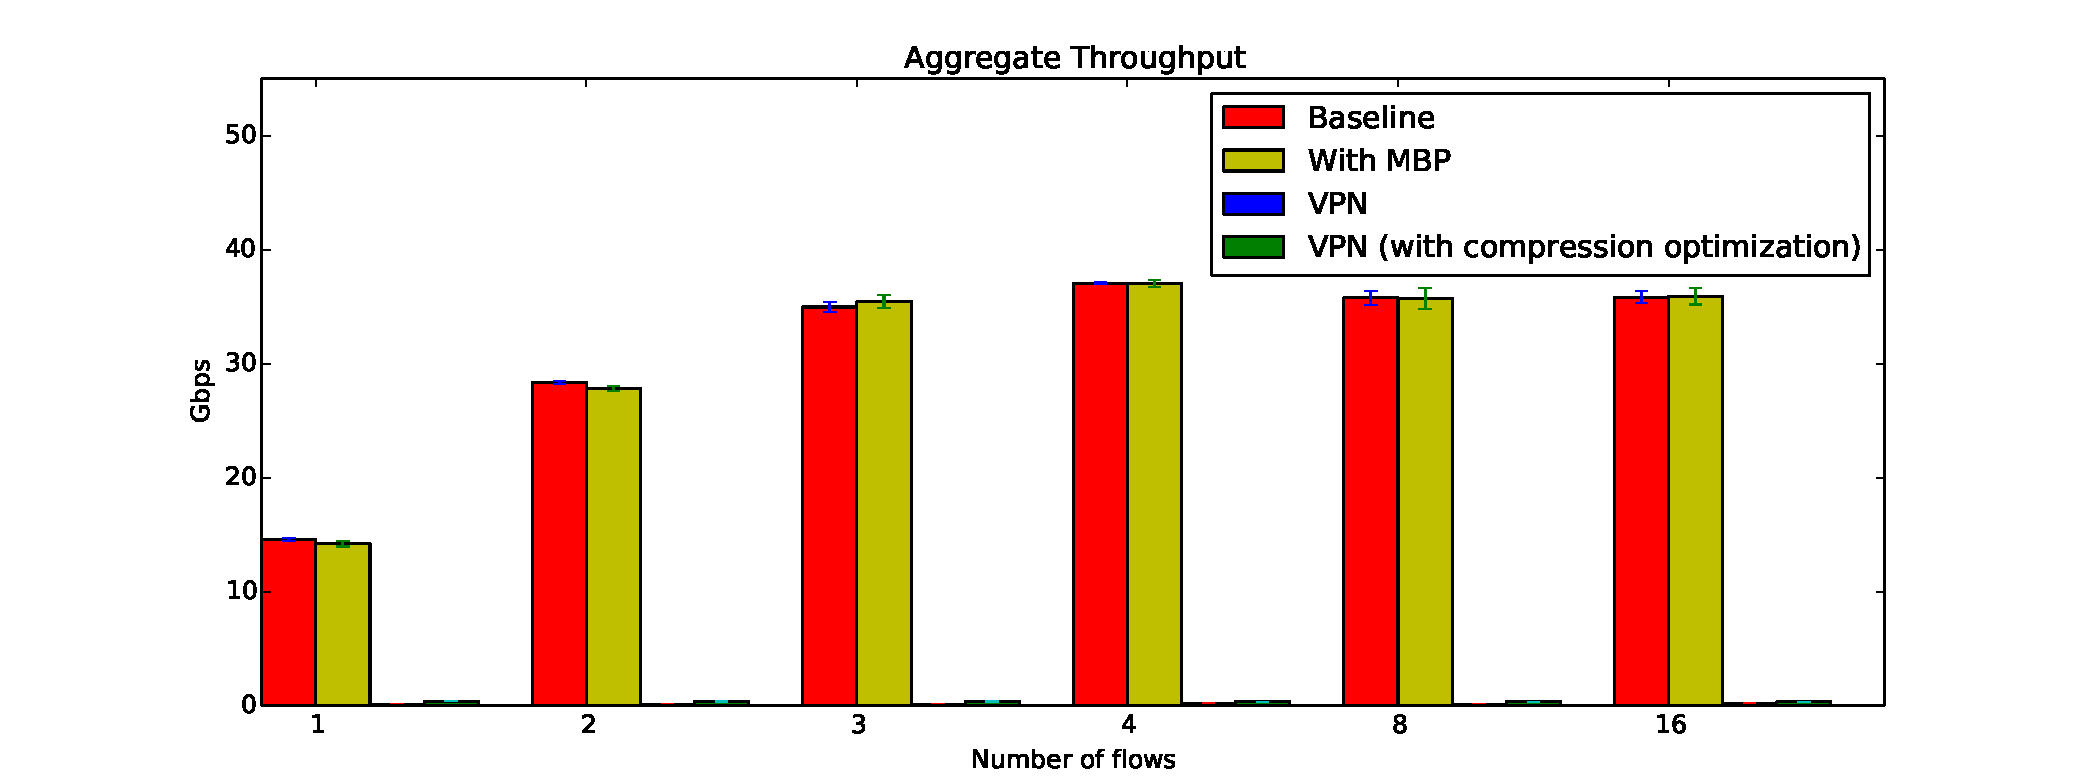
\includegraphics[width=\linewidth]{figures/throughput.pdf} 

\caption{ Throughput  of  different approaches.}\label{throughput}
\end{figure*}

Figure~\ref{throughput} shows the throughput measurements for the five
different scenarios:  \system, baseline,  VPN, VPN+OP,  and  OVS.  The
results show the  \system kernel-module data plane  implementation can
sustain $14.2$ Gbps on  a single core,  and it scales linearly  to the
number of  cores, reaching  $37.1$ Gbps at  its peak.   The difference
betweek the peak throughput and 40Gbps is because {\tt iperf} measures
the throughput  at  the  application    layer, i.e., packet    headers
(TCP+IP+Ethernet) are not  included in the computation.   The baseline
case yields  a  throughput of  $14.6$  Gbps on  a  single core, so the
kernel module overhead  is under  $3\%$ in  the  worst case.   As  the
number of flows    increases,   more cores  are involved   in   packet
processing and the gap between \system  and the baseline shrinks until
it becomes negligible.  The reason  is that interrupts per core happen
less frequently and the link  bandwidth becomes the bottleneck instead
of the CPU. We envision if  we increase the NIC  bandwidth to 100 Gbps
or higher,  the gap will stay the   same and the throughput  will grow
linearly before    the link  bandwidth   or the   PCI bus  become  the
bottleneck.

We initially observed inconsistent results  for four flows because the
default  hash  function (Toeplitz  hash)   of the NIC  driver  was not
spreading  well the flows  into different  cores.   We had to apply  a
minor tweak  on the NIC driver to  get a  better distribution of flows
into cores.  When  the number  of  flows is small, the  driver  manual
recommends the  change of the Toeplitz hash  function to  a simple XOR
function to avoid   flow colliding on the   same core~\cite{mellanox}.
After we changed the   hash function, we observed consistent  results.
The same configuration was used for the five scenarios.

The throughput results for the other three scenarios are also depcited
in Figure~\ref{throughput}. We compare our approach with off-the-shelf
VPN-encapsulation mechanism,  which is used in APLOMB~\cite{Aplomb} to
achieve its redirection.  Not surprisingly,   VPN uses encryption  and
thus offers much lower  throughput.  OpenVPN~\cite{openvpn}, which  is
used in APLOMB, achieves  less than $400$ Mbps on  a single core, even
with the compression  optimization.  Current OpenVPN does  not support
multi-threading and is not  able  to take  advantate of  the  multiple
cores  on  the machines.  Even  if  multi-threading is incorporated in
OpenVPN in the future and assuming it will scale linearly to 16 cores,
it will be able to offer only 17\% of the maximum throughput.

OVS results.

%It is well   documented that when the  number  of flows is  small, the
%default  hash function of   the NIC driver   (Toeplitz hash)  does not
%perform well and  different flows  are mapped to   the same core.   We
%changed the   hash  function to a    simple XOR function,  which  is a
%recommendation of the driver manufacturer~\cite{mellanox}.

\begin{figure}[ht]
\centering
% 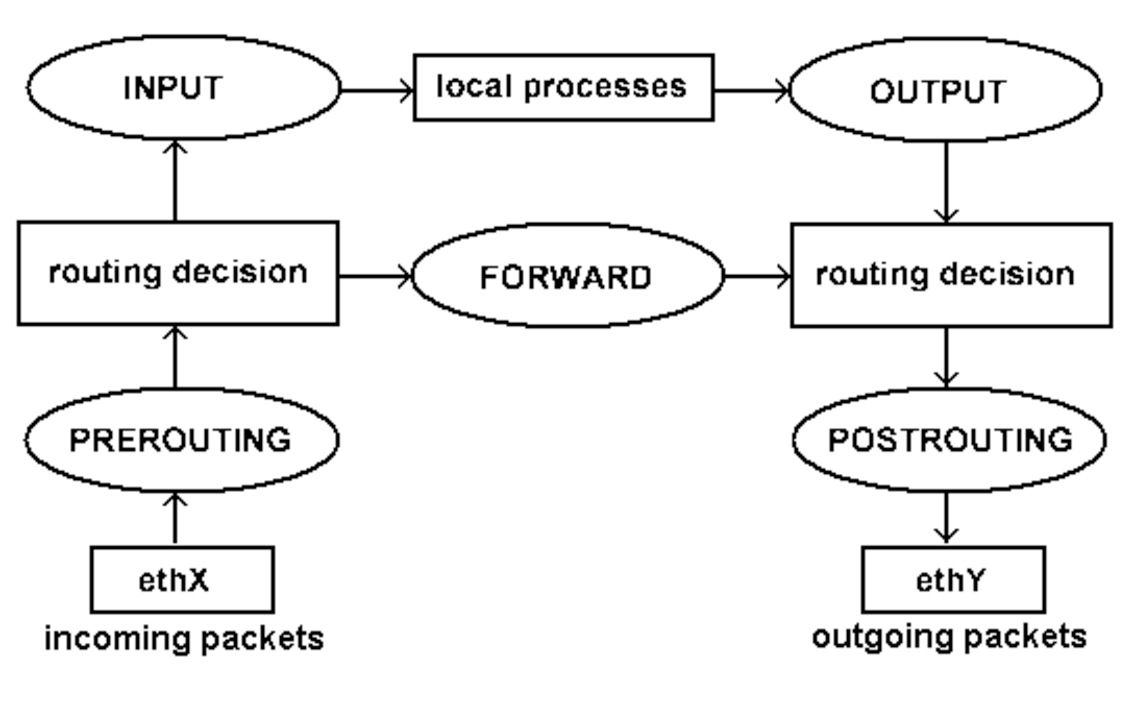
\includegraphics[scale=0.25]{figures/netfilter.pdf} 
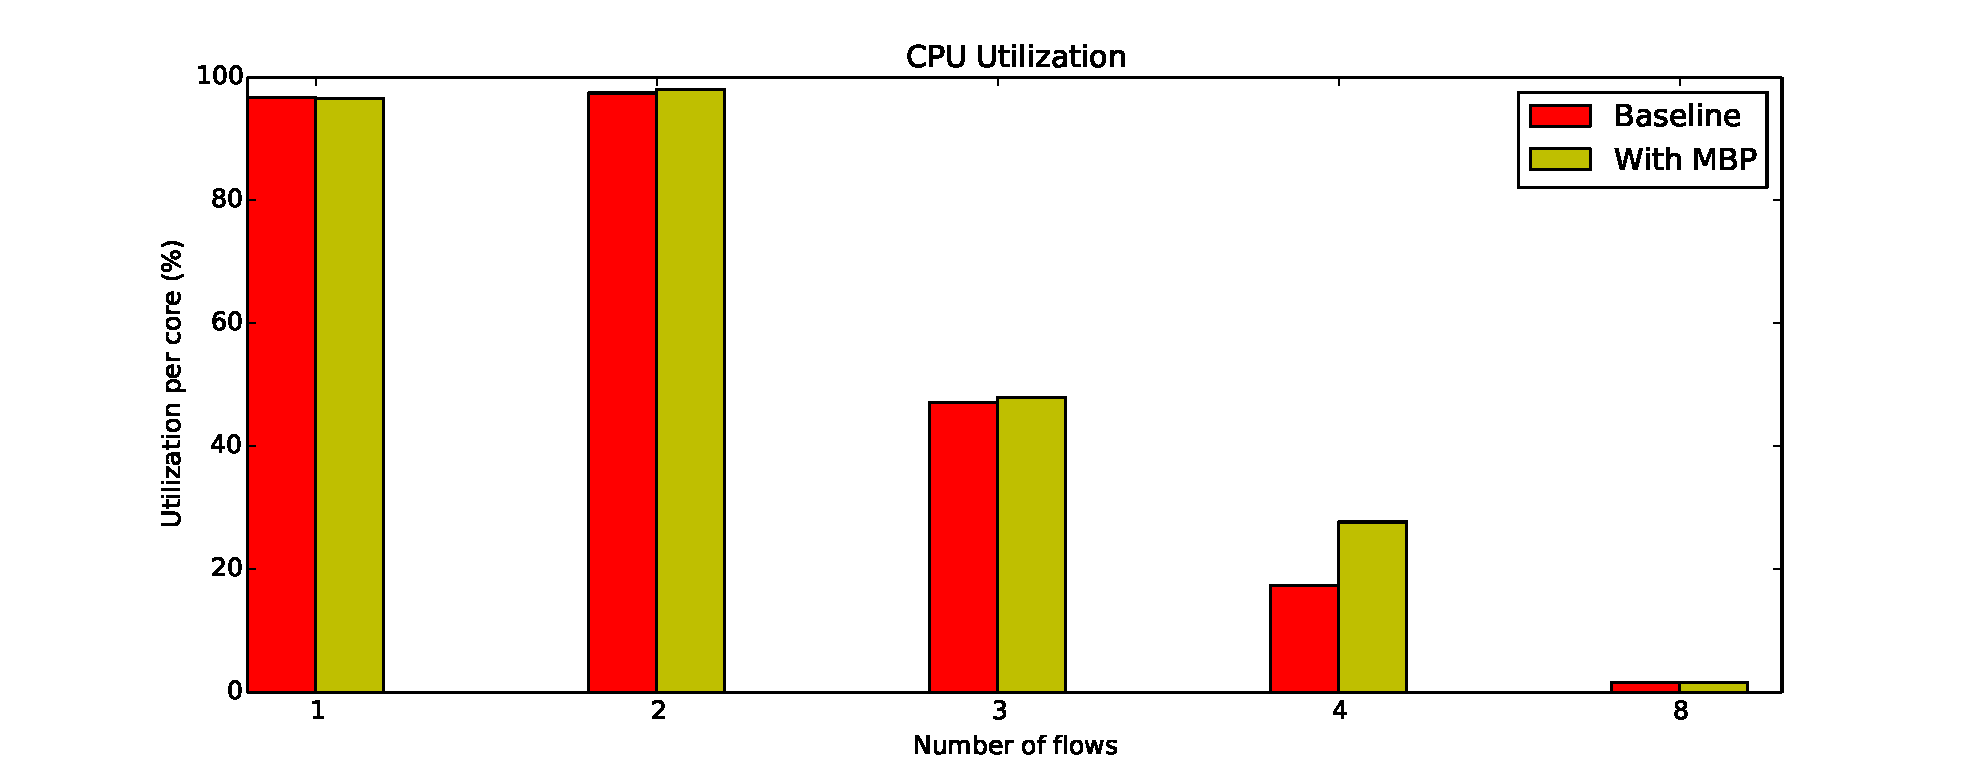
\includegraphics[width=\linewidth]{figures/CPU.pdf} 
% 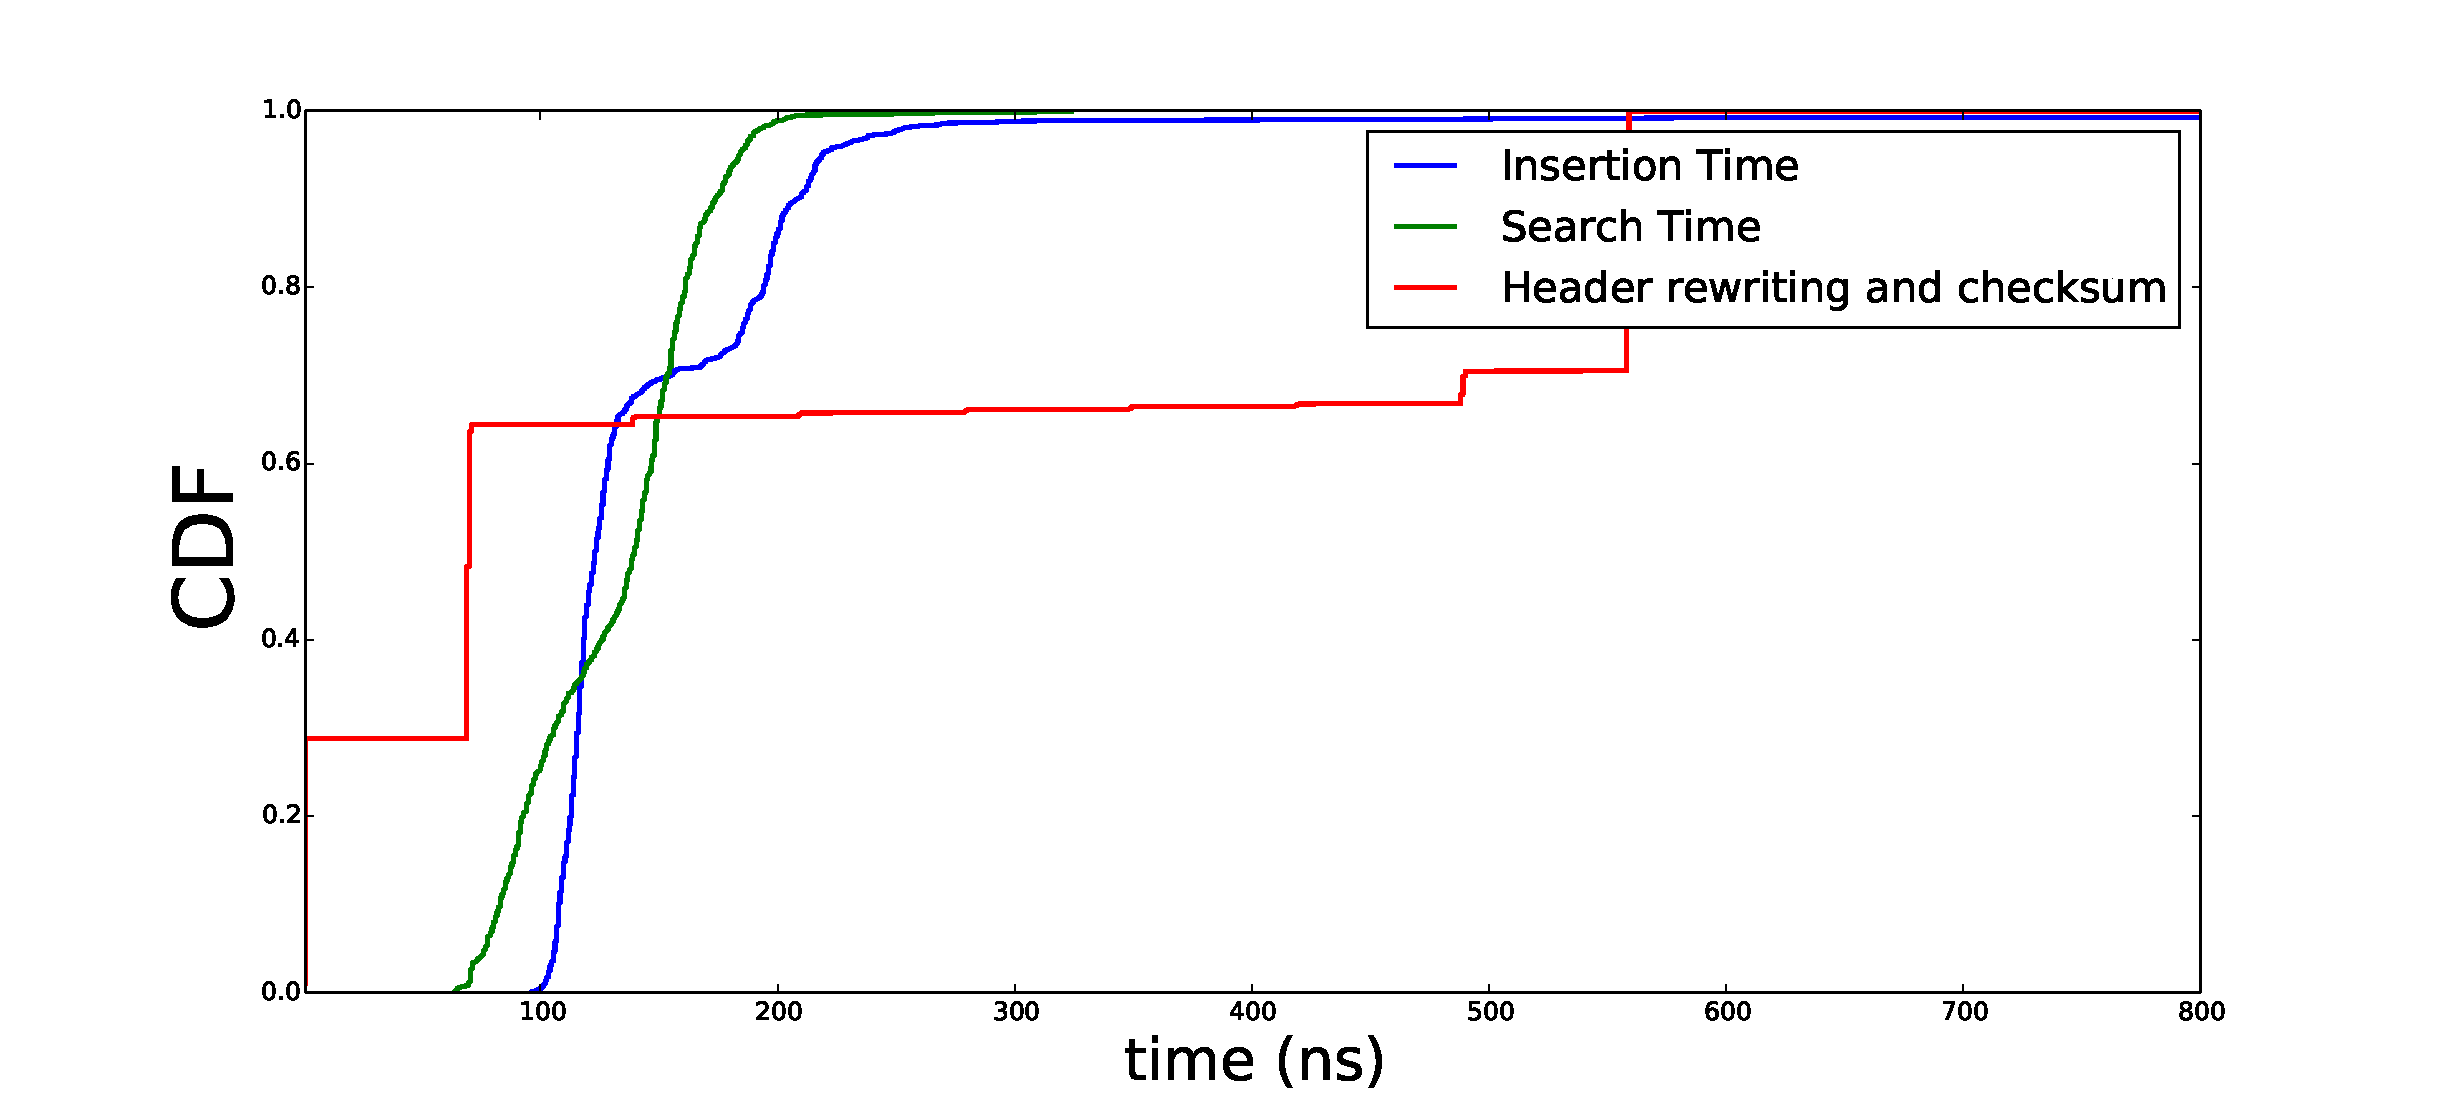
\includegraphics[width=\linewidth]{figures/cdf.pdf} 
\caption{\small Average CPU utilization in stress test. Note we only include the cores that are interrupted by the NIC.}\label{cpu-utilization}
\end{figure}

Figure~\ref{cpu-utilization}   shows  the    CPU  utilization  of  the
middlebox in the same experiments.  Note that since the middlebox acts
as a software  router without the  kernel module,  it also consumes  a
certain  amount  of CPU  cycles.   The highest difference between  the
baseline and the system  lies  in the setting  of   4 flows,  the  CPU
utilization  for \system  is 10\%   higher than that  of the  baseline
(27.6\% versus 17.2\%), but under most circumstances the gap is within
2\%. One thing worth noting is that  as the number of flows increases,
the  CPU utilization per core  plummets, our explanation is that since
the testbed machine has 16 cores and 32  hyper-threads, it spreads out
quite evenly, and the CPU utilization scales linearly at high load but
it is not the case at low load  (e.g., 1M packets/s causes much higher
CPU utilization than 500K packets/s).

The  experimental   results    are  promising   and   prove  that  the
kernel-module data plane implementation can offer very high throughput
at the cost of modest increase of CPU utilization.


\subsubsection{Microbenchmarks}

The kernel-module implementation of the data plane includes three main
functions:  (i) table lookup for   vertical and horizontal NATs;  (ii)
header rewriting and re-checksum; and (iii) rule installation.

We also
have  a  few  optimizations in  the  data-plane  implementation (e.g.,
partial checksum to reduce CPU cycle, a small hash  table to fit in L3
cache)    result in an extremely  efficient   system with   a very low
overhead.

We conducted a microbenchmark to see the delay different functions add
to the  system. We insert 100K  rules  in the  kernel  hash table, and
conducted 100K  lookup. We also  microbenchmarked the header rewriting
and partial checksum of  the data packets.   We had the  two following
methods to  eliminate Linux timer's  overhead: (i) batch  and time the
insertion  and lookup for every one  hundred rules; (ii)  get the pure
timer lookup time and then subtract that base number. The result shows
that lookup, insertion and header rewriting takes on average 131, 251,
and 214 ns, this  gives us $\approx  $  2.8M packets per seconds  with
lookup and header rewriting, this is  equivalent to 33.6 Gbps per core
with MTU of 1500 Bytes.

\begin{figure}[ht]
\centering
% 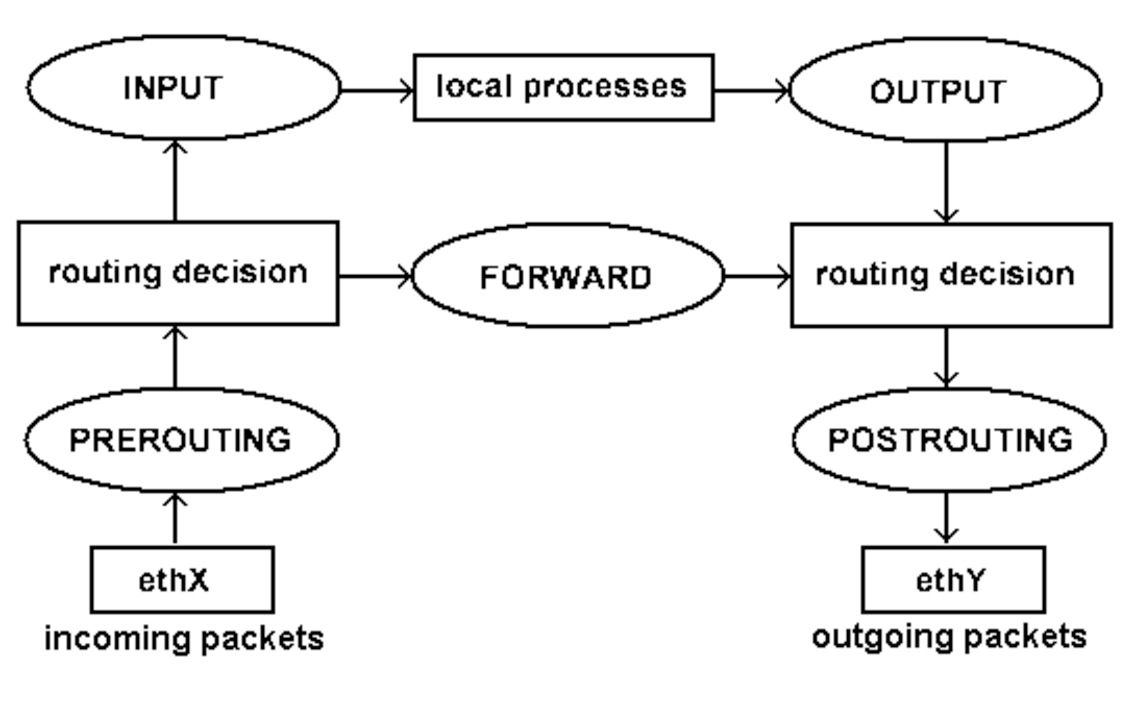
\includegraphics[scale=0.25]{figures/netfilter.pdf} 
% 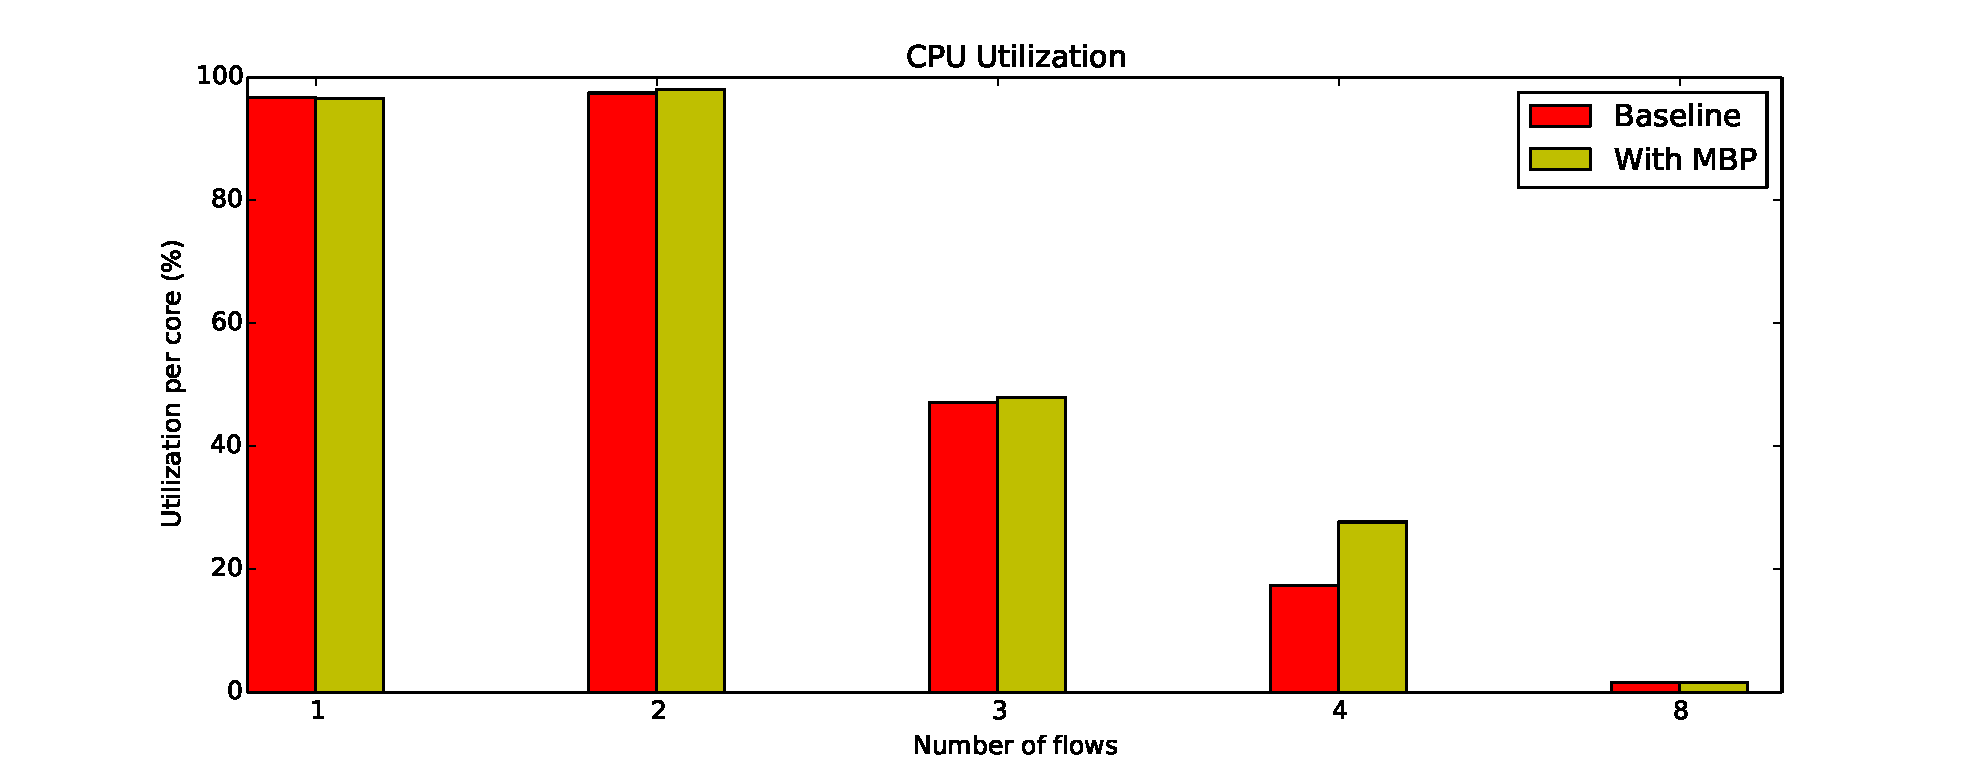
\includegraphics[width=0.53\linewidth]{figures/CPU.pdf} 
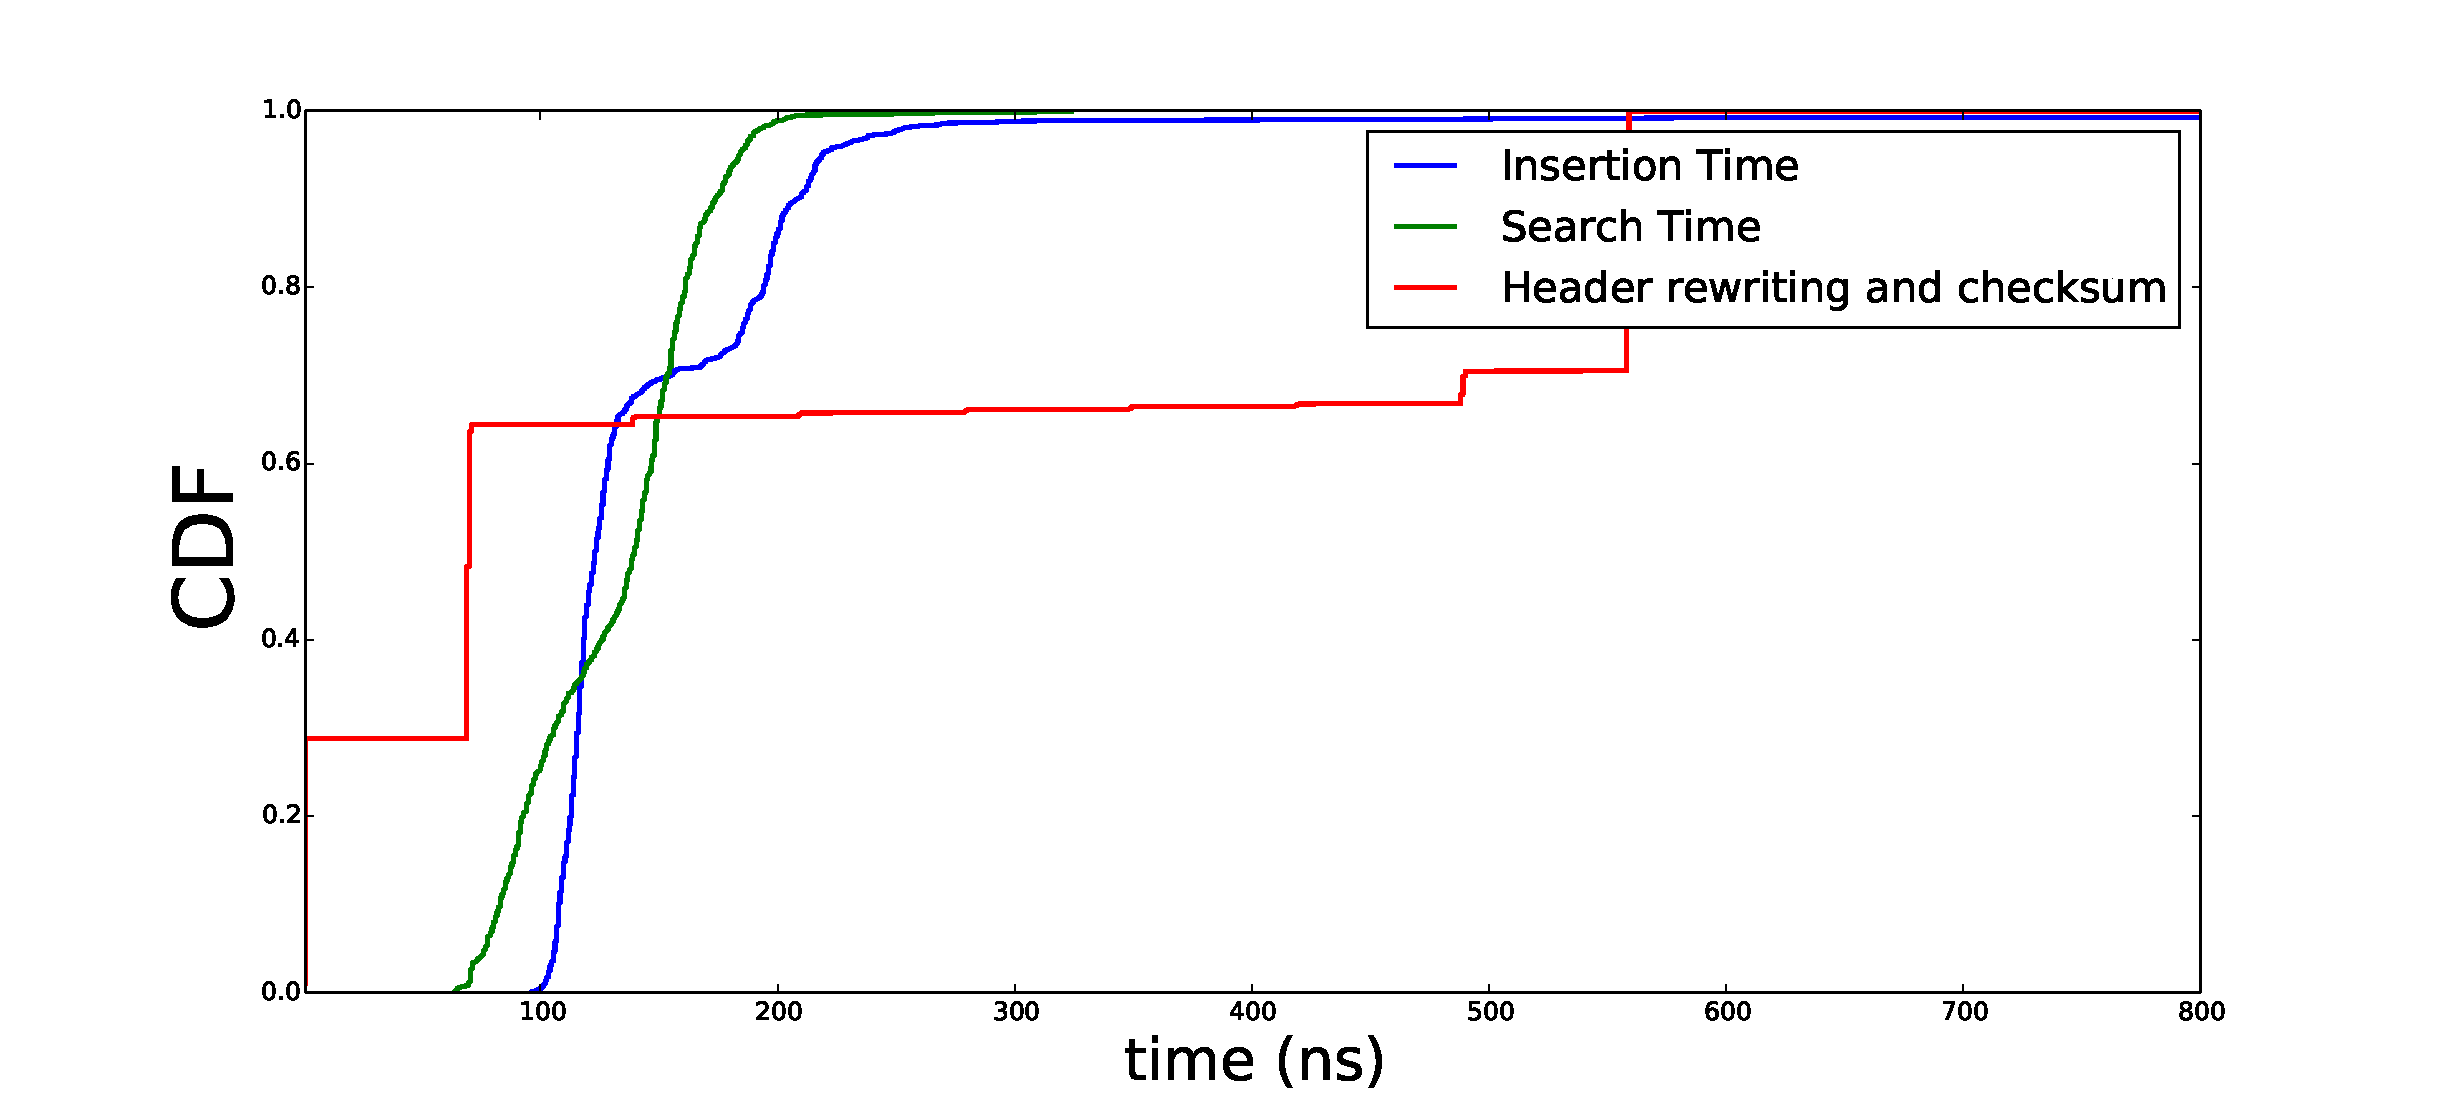
\includegraphics[width=\linewidth]{figures/cdf.pdf} 
\caption{\small Time CDF for different functions}\label{microbenchmark}
\end{figure}
% 



%We also  changed the NIC's ring buffer
%hash   function to an   XOR   hash function   to avoid  core interrupt
%collision, since   the default hash   function  is designed  for large
%number of flows, we see noticeable collision,  i.e., hash two flows to
%the same ring buffer when the number is small.
%The gap is closing as  we increase  the number of
%flows,  sice it  incurs    less frequent  interrupts   per core  (the
%frequency of  per-core interrupt for 4 flows  with 9 Gbps  per flow is
%66\% of a single flow with 14.5 Gbps), and thus the stress per core is
%lighter. 


%One interesting  observation is that when there   are three flows, the
%system offers a higher throughput than the baseline. The reason behind
%it  is that the ``extra  work'' tends to keep  the cores busy and thus
%gets more  CPU  cycles for  processing.  The competing flows from  TCP
%congestion control may also affect the throughput.

\subsection{Latency}

We evaluate our system's latency in the  following order: (i) how much
overhead it has  for a super-session setup? (ii)  how much overhead it
has during an update while preserving  different properties. We choose
setting (i) testbed  since it is closer to  a real  enterprise network
w.r.t.  round trip time and switch  buffer size (queuing delay). Since
\system  is  per-flow based  operation, the number  of flows  does not
affect per-flow latency.


\subsubsection{Three-Way handshake}
\label{sec:3way-handshake}
% \kelvin{will add more stuff, like three hops, 4 hops and 5 hops, but do get the idea of how to do it now, three hops values are 426.5 28.7515216989, 464.5 22.8527897641, 688.1 24.6473122267}

We first measure the latency for  session establishment, in a topology
of three  hops (client -  middlebox -  server). We have  two different
implementation, (i)  out of  band UDP  ahead   to TCP handshake,  (ii)
piggyback  TCP handshake   at  the   payload. Not surprisingly,    TCP
piggyback can   greatly reduce the extra    latency due to propagation
delay, with a modest increase less than $40 \mu $s. On the other hand,
out-of-band UDP incurs $688\mu$s delay ahead of TCP handshake.

\begin{figure}[ht]
\centering
\includegraphics[width=\linewidth]{figures/latency_threeway.pdf} 
\caption{\small Latency for session establishment}\label{threeway}
\end{figure}


\subsubsection{Flow Migration}

\system supports flow  migrations with various properties.  We measure
the time  interval for   such  an update   with a  loss-free,   packet
order-preserving,  and  substream order  preserving.  We  also created
artificial   packet  reordering in  the  case   of  byte stream  order
preserving during an update.


We run our experiments in a topology with four machines (A,B,C,D) with
two paths  (A - B -  D) and (A  - C - D)  that  each consists of three
hops. Client and server are at A and D. The goal of the flow migration
is   to replace  middlebox B   with  D. We   measure  the latency  for
migrations with (a) loss-free (LF), (b) order-preserving (OP), and (c)
substream separation   and order  preserving  (SS+OP)  properties. The
latency are  evaluated under a full  load on a  network with all 1Gbps
links. All tests are run in TCP Cubic.

\begin{figure}[ht]
\centering
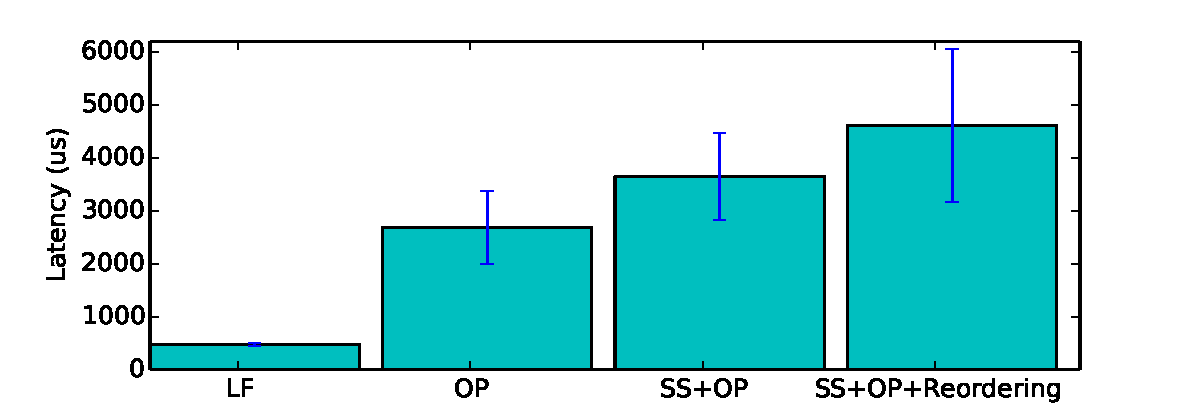
\includegraphics[width=\linewidth]{figures/latency_four_types.pdf} 
\caption{\small Latency of flow migration with loss-free (LF), packet order-preserving (OP), substream-separation and order-preserving (SS+OP), and substream-separation and order-preserving (SS+OP) with an artificial reordering. }\label{fig_update_latency}
\end{figure}


We summarize  the  latency result  on Figure~\ref{fig_update_latency}.
During a loss-free migration, the old path  is saturated; however, the
new path  is idle during  a subsession  setup and thus  has the lowest
latency. During a  order  preserving migration,  \system  has to  send
subsession setup on the new path and a marking  packet right after the
end of data packets on the old path; the higher  latency is mostly due
to the queuing delay on the old path.  During substream separation and
order preserving migration, besides the queuing delay, the ACK message
may also be delayed from the receiving side, e.g.,  the extra time for
TCP to process  the byte stream  and generate an  ACK. Since we rarely
see packet reordering in the testbed during an update, we artificially
created a  packet  reordering  via dropping a    packet  with a  lower
sequence number in the kernel, which triggers  a retransmission of the
packet  with a lower  sequence number after  the  packet with a higher
sequence number.

The results demonstrate that the  system can deal with flow migrations
in  the order  milliseconds.   This can greatly  facilitate   the flow
migration during an NF insertion, removal and hot-standby replacement.
NF      state  migration      can     happen  within     hundreds   of
milliseconds~\cite{OpenNF, splitmerge},  here results show that a flow
migration should no  longer be considered a bottleneck  in the case of
NF state  and corresponding flow  migration. A more detailed breakdown
is in Table~\ref{latencycomp}.

\begin{table}[ht]
\centering
\small
\begin{tabular} {|l |c | c| c|}

\hline
 &LF& OP &SS+OP \\ \hline 
% &~\cite{SIMPLE,FLOWTAGS, OpenNF}& ~\cite{CoMB, splitmerge}& ~\cite{ Aplomb,DOA,I3} & ~\cite{OVS, Netfilter} & \\ \hline

Split/Merge
\footnote{\scriptsize at packet rate 37.5 kpps, time are consumed across flow migration and state migration} 
		&~500ms& {\small no support}& {\small no support} \\ \hline
Dionysus
\footnote{\scriptsize Large-scale networks}
	      &600-1200ms &{\small no support}&{\small no support}   \\ \hline
OpenNF
\footnote{\scriptsize flow update time at packet rate 2.5-10 kpps} 
	       & 84ms& 96ms&{\small no support}\\ \hline
\system
\footnote{\scriptsize at packet rate 80 kpps (1 Gbps)} 
	    & 0.5ms & 2.7ms&3.6ms \\ \hline

\end{tabular}
\caption{Comparison with other dynamic middlebox and flow migration systems}\label{latencycomp} 
\end{table}

